\section{Aufbau und Durchführung}

  
\noindent
Der Versuchsaufbau ist schematisch in Abbildung \ref{img:aufb} dargestellt. 
Er besteht aus einer Halogenlampe, deren Lichtstrahl über eine Linse parallelisiert wird und dann auf einen Lichtzerhacker trifft.
Anschließend wird der Strahl mit Hilfe eines Glan-Thompson-Prismas aus Kalkspat linear polarisiert. 
Der Winkel, unter dem der Strahl polarisiert wird kann über ein Goniometer eingestellt werden.
Im Strahlengang hinter dem Prisma werden die zu untersuchenden $\ce{GaAs}$- oder $\ce{InGaAs}$-Proben in den Luftspalt eines Elektromagneten eingebracht.
Der Magnet ist dabei an eine regelbare Konstantstromquelle angeschlossen. 
Hinter dem Magneten und der Probe ist ein austauschbarer Interferenzfilter im Strahlengang angebracht.
Anschließend wird der Strahl von einem weiteren Glan-Thompson-Prisma in zwei orthogonal polarisierten Strahlen aufgespalten. 
Diese werden auf zwei Photozellen fokussiert, deren Ausgangssignale an einem Differenzverstärker anliegen. 
Der Differenzverstärker gibt eine Spannung aus, die proportional zur Differenz der Eingangsspannungen ist. 
Dies bedeutet, dass das Signal für identische Phase und Amplitude der Eingangspulse verschwindet.\\
Dessen Ausgangssignal liegt an einem Selektivverstärker an. 
Dieser verstärkt Signale in einem ausgewählten Frequenzbereich, welcher auf die Frequenz des Lichtzerhackers abgetimmt wird ist.
Auf diese Weise wird der Einfluss des Signalhintergrunds der Photowiderstände minimiert. 
Der Selektivverstärker liegt an einem Oszilloskop an, welches als Nulldetektor verwendet wird. Damit ermittelt man das Nullsignal des Differenzverstärkers.\\


\begin{figure}[H]
    \centering
    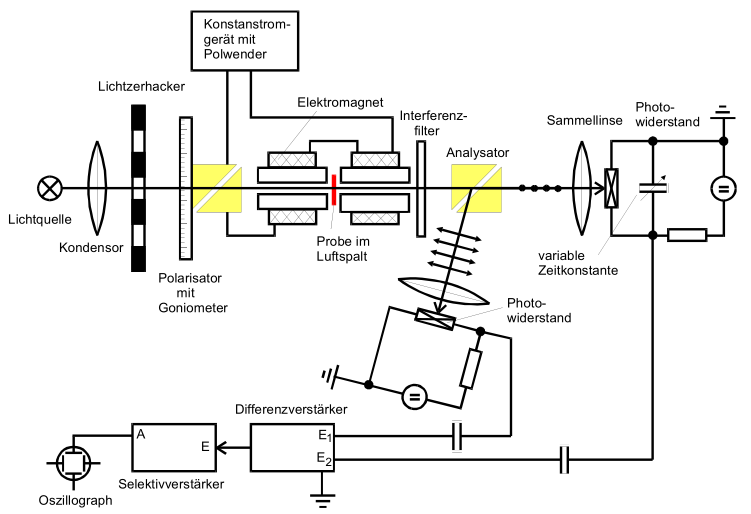
\includegraphics[width=0.7\textwidth]{latex/images/Aufbau.PNG}
    \caption{Der schematische Versuchsaufbau der zur Untersuchung des Faraday-Effektes verwendet wird \protect \cite{V46}.}
    \label{img:aufb}
\end{figure}



\noindent
Zuerst wird der Aufbau justiert. Dafür werden Probe, Interferenzfilter sowie das Gehäuse der Photowiderstände entfernt.
Anschließend wird überprüft ob der Polarisationsprisma orthogonal auf der Ausbreitungsrichtung des Strahls steht.
Dafür muss bei Rotation des Prismas eine der vom zweiten Glenn-Thompson-Prisma ausgegebenen Intensitäten zum Verschwinden gebracht werden können.
Ist dies nicht erfüllt muss der erste Prisma vorsichtig gedreht werden.\\
Anchließend wird überprüft, ob die Ausgangsstrahlen des zweiten Prismas auf die beiden Photowiderstände abbilden und 
ob durch Drehung des ersten Prismas die Intensität vollständig zwischen den beiden Widerständen umgeschaltet werden können.
Um dies zu gewährleisten, können die Photozellen verschoben werden.\\
Zuletzt wird der Selektivverstärker eingestellt. 
Dafür werden der Differenzverstärker, der Selektivverstärker und das Oszilloskop, wie in Abbildung \ref{img:aufb} dargestellt, angeschlossen.
Dann werden der Lichtzerhacker, sowie der Selektivverstärker auf auf $\SI{450}{\hertz}$ gestellt. 
Des Weiteren wird der Gütefaktor $Q = 100$, welcher ein Maß für die Durchlassbreite ist, eingestellt. 
Außerdem werden die drei Frequenzstellknöpfe so eingestellt dass, das am Oszilloskop gemessene Signal maximal wird.
Zuletzt wird ein Interferenzfilter in den Aufbau eingebracht und überprüft ob minimale Intensitätsamplituden sich bei Drehung 
des ersten Polarisationsprismas mit einer Periode von $\SI{90}{\degree}$ wiederholen.\\\\

\noindent
Für die Messung wird eine der drei Proben und einer der Interferenzfilter in den Aufbau eingebracht.
Nun wird das Magnetfeld auf den maximalen Wert eingestellt und der Winkel so justiert, dass die Intensitätsamplitude am Oszilloskop minimal wird.
Der damit korrespondierende Winkel wird vom Goniometer abgelesen und notiert. Dann wird das Magnetfeld umgepolt und das Vorgehen wiederholt.
Dies wird erst für 9 Interferenzfilter von $\SI{1.06}{\micro\meter}$ bis $\SI{2.65}{\micro\meter}$ durchgeführt und dann noch einmal für die anderen Isotope wiederholt.\\
Zuletzt wird die Magnetfeldstärke in der Lücke zwischen den Magneten ausgewertet. 
Dafür wird dort eine Hall-Sonde eingebracht und über einen Bereich von $d = \SI{20}{\milli\metre}$ mit $\increment d = \SI{1}{\milli\metre}$ das Magnetfeld ausgemessen.